\section*{Figures}

\listoffigures

\clearpage

\begin{figure}%[tbhp]
\centering
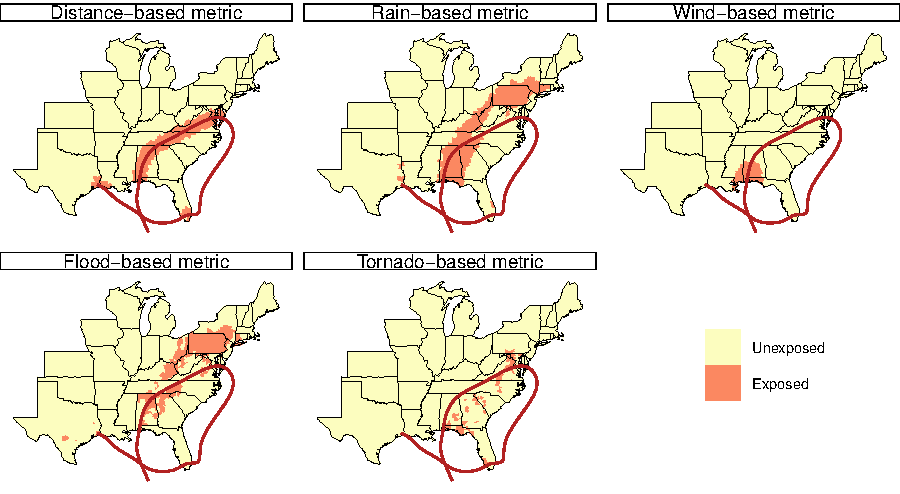
\includegraphics[width=16cm]{ivanonly}
\caption{Counties classified as exposed to Hurricane Ivan (2004) under each
exposure metric (Table 1). The red line shows the track of Hurricane Ivan 
based on the revised Atlantic hurricane database (HURDAT2 \cite{landsea2013}).
Similar maps for other large-extent storms are given in Fig. S3.}
\label{fig:ivanexposure} 
\end{figure}

\clearpage

\begin{figure}%[tbhp] 
\centering 
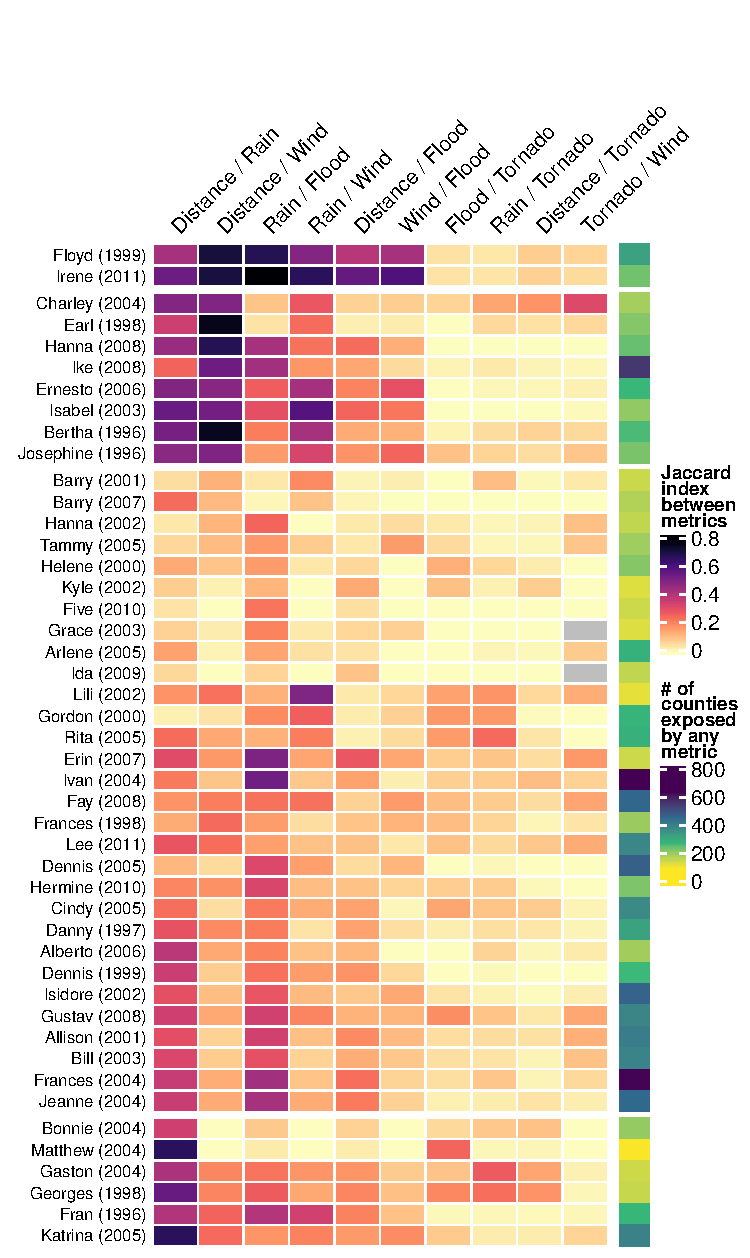
\includegraphics[width = 0.6\linewidth]{jaccard_heatmap} 
\caption{Heatmap of Jaccard index values for
specific exposure metric pairs within storms. Only storms between 1996 and 2011,
and for which at least 250 counties were exposed based on at least one metric,
are included. The color of each cell within the main heatmap indicates the value
of the Jaccard index (proportion of counties classified as exposed by both
metrics out of storms classified as exposed by either metric) for a given pair
of metrics for a given storm. Storms are displayed within clusters that have
similar patterns in county-level exposure agreement for metric pairs, based on
hierarchical clustering using the complete link method
\cite{murtagh2012algorithms} (i.e., storms in the same cluster tend to have
similar patterns for the pairwise strength of agreement among metrics); columns
are also ordered based on hierarchical clustering. The colors to the right of
the main heatmap for each storm indicate the total number of counties classified
as exposed to the storm by any of the five metrics, providing an estimate of
storm extent. Maps are available showing the counties identified as exposed
under each of five metrics for the widest-extent storm in each cluster:
Hurricane Ivan (2004) (Fig. \ref{fig:ivanexposure}) and Hurricanes Floyd (1999),
Lee (2011), Cindy (2005), and Katrina (2005) (Fig. S3).} 
\label{fig:jaccard}
\end{figure}

\clearpage

\begin{figure}%[tbhp] 
\centering
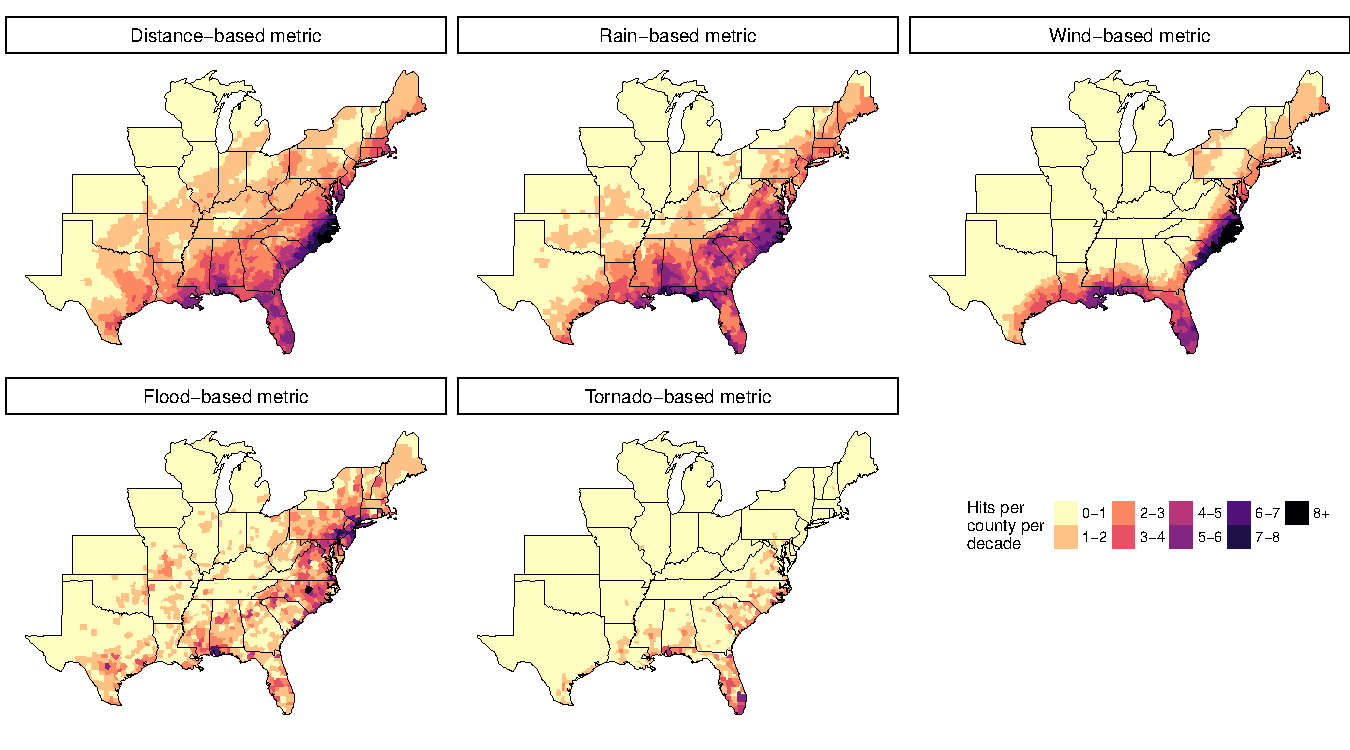
\includegraphics[width=15cm]{averageexposureonly} 
\caption{Average number of storm exposures per decade in U.S. counties for 
each exposure metric. The criteria behind each of the five metrics is given 
in Table \ref{tab:exposuremetrics}. The years used to estimate these averages 
are based on years of available exposure data (distance and wind: 1988--2015; 
rain: 1988--2011; flood and tornado: 1996--2015). Similar patterns persist when
analysis is restricted to years with all exposure data available (1996--2011;
Fig. S5).} 
\label{fig:averageexposure} 
\end{figure}